\chapter{Introduction}
\label{Introduction}
\thispagestyle{fancy}

\section{Présentation du produit}
\label{Introduction:Présentation du produit}
On présente ici de manière succincte l'architecture Hardware du robot Pepper afin de se familiariser avec les différents éléments du système avec lesquels on sera susceptible de travailler durant la mise en œuvre de ce projet.  

\subsection{Les actionneurs}
\label{Introduction:Présentation du produit:Les actionneurs}
\subsubsection{Les moteurs}
\label{Introduction:Présentation du produit:Les actionneurs: Les moteurs}
Le robot Pepper est constitué de 20 moteurs dont il est possible de contrôler la position et la rigidité (figure \ref{fig:Répartition des actionneurs de Pepper})
\begin{description}
	\item [Tête:] 2 moteurs pour les mouvements de lacet (HeadYaw) et de tangage (HeadPitch)
	\item [Bras:] 4 moteurs par bras, répartis de la manière suivante: 
	\begin{description}
		\item [Épaule:] 2 moteurs pour les mouvements de tangage (ShoulderPitch) et de roulis du bras (ShoulderRoll).
		\item [Coude:] 2 moteurs pour les mouvements de roulis (ElbowRoll) et de lacet (ElbowYaw) de l'avant-bras.
	\end{description}
	\item [Main:] 1 moteur pour le mouvement de lacet du poignet (WristYaw) et 1 pour le mouvement d'ouverture et de fermeture de la main (Hand).
	\item [Hanche:] 2 moteurs pour le mouvement de roulis (HipRoll) et de tangage (HipPitch) du buste.
	\item [Genoux:] 1 moteur pour le mouvement de tangage (KneePitch) du haut du corps.
	\item [Roues:] 3 moteurs pour les mouvements de rotation de chacune des 3 roues omnidirectionnelles (WheelB, WheelFR et WheelFL).
\end{description}

\begin{figure}[h]
	\centering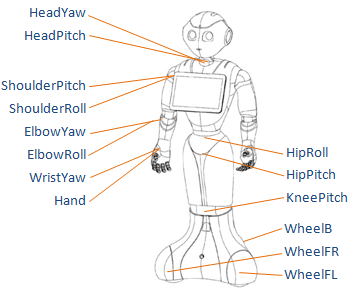
\includegraphics[height=7cm]{images/pepper_motors.png}
	\caption{Répartition des actionneurs de Pepper}
	\label{fig:Répartition des actionneurs de Pepper}
\end{figure}

\subsubsection{Les LEDs}
\label{Introduction:Présentation du produit:Les actionneurs: Les leds}
Les LEDs placées sur les épaules de Pepper, autour de ses yeux et de ses oreilles permettent d'obtenir un certain nombre d'informations sur son état. Par exemple, des LEDs bleues en rotations autour des yeux indiquent que le robot écoute.

\subsection{Les capteurs}
\label{Introduction:Présentation du produit:Les capteurs}
Pepper intègre également une multitude de capteurs. Certains d'entre eux sont utilisés pour s'assurer du bon comportement des parties mécaniques du robot, ou pour réaliser du contrôle-commande. D'autres capteurs sont en revanche intégrés sur le robot afin que l'utilisateur puisse interagir avec lui (tableau \ref{tab: Les différents capteurs de Pepper}).

\begin{table}[h]
	\begin{tabular}{ | p{3cm} | p{4cm} | p{7cm} | }
		\hline
		Capteur & Position & Description \\
		\hline
		Capteurs liés aux actionneurs & sur les moteurs & Chaque moteur du robot est lié à 3 capteurs, qui donnent des informations sur la valeur du courant délivré au moteur (A), la température du moteur (\degres C) et la position du moteur. \\
		\hline
		Capteurs tactiles & 1 sur chaque main, 3 sur la tête & Permet à l'utilisateur d'interagir avec le robot en le touchant.	\\	
		\hline 
		Les boutons & 1 bouton poussoir sur le buste, 3 bumpers sur la base & Les bumpers permettent au robot de détecter s'il rencontre un obstacle à proximité immédiate. Le bouton du buste permet quant à lui d'allumer le robot et de modifier le mode dans lequel il est (autonome, veille). \\
		\hline 
		Centrale inertielle & 1 dans le buste, 1 dans la base & Informe sur la position et l'orientation du robot, ainsi que la vitesse et l'accélération. \\
		\hline
		Sonars & 2 sonars à l'avant et l'arrière de la base & Permet de détecter la présence d'un objet situé au delà de 65 cm du robot. \\
		\hline 
		Capteurs batterie & batterie & Renseigne sur le courant et la tension délivrés, le pourcentage de charge et la température. \\
		\hline
		Capteurs infra-rouges & 2 sur la base &  Permet de détecter la présence d'un objet situé entre 0 et 50 cm du robot. \\
		\hline
		Lasers & 6 lasers sur la base du robot & Permet de détecter la présence d'un objet \\
		\hline 
	\end{tabular}
	\caption[Les différents capteurs de Pepper]{Les différents capteurs de l'architecture sensorielle de Pepper}
	\label {tab: Les différents capteurs de Pepper}
\end{table}


\section{Expression du besoin}
\label{Introduction:Expression du besoin}
L'extension du marché visée par Aldebaran pour Pepper s'accompagne d'une montée en puissance de la production. Afin de la guider, des outils de vérification des produits en fin de ligne de production sont mis en place. Parmi eux, on retrouve le "Filtering Test" qui consiste à réaliser une série de tests durant six heures. Il vise à stresser l'ensemble des parties mécaniques du robot afin de faire ressortir d'éventuelles erreurs.

 \subsection{DExTER et MEIGUI}
 \label{Introduction:Expression du besoin:DExTER et MEIGUI}
 L'équipe de qualification hardware de Pepper a mis au point deux outils qui permettent de réaliser ces test et d'analyser les erreurs apparues.
 \begin{description}
 	\item[MEIGUI :] Le Filtering Test est réalisé grâce à MEIGUI. Celui-ci fait effectuer au robot un ensemble de mouvements qui permettent de stresser ses parties mécaniques. Si une anomalie survient lors du déroulement du test, les différentes données relatives à l'état des systèmes mécaniques et électroniques de Pepper sont enregistrées dans un fichier journal (e.g. température des fusibles, valeur des accéléromètres, etc.). 
 	\item[DExTER :] Afin d'identifier les causes de l'apparition de problèmes sur le robot, un certain nombre d'hypothèses sont émises à partir de l'étude des données du fichier log. Pour cela, on s'appuie sur l'utilisation d'un autre outil, DExTER, qui permet de visualiser les données du fichier log et d'obtenir des informations sur ces dernières (date d'apparition de l'erreur, nombre d'erreurs apparues, etc.).
 \end{description}
 
\subsection{Hiérarchisation des erreurs}
\label{Introduction:Expression du besoin:Hiérarchisation des erreurs}
Pour gérer au mieux les anomalies, celles-ci sont hiérarchisées en deux catégories: les \emph{errors name} et les \emph{root causes}.
\begin{description}
	\item [Error name] Cela correspond à l'erreur visible, i.e. la conséquence liée à une anomalie hardware ou software. Par exemple, il peut s'agir de la chute du robot. 
	\item [Root cause] Il s'agit de l'anomalie en elle même, i.e. la cause ayant entraînée l'apparition d'une \emph{error name}. Si l'\emph{error name} est la chute d'un robot, la \emph{root cause} peut par exemple être la détérioration d'un engrenage de la hanche.
\end{description} 

En suivant la logique exprimée par ces définitions, une \emph{error name} peut être constituée d'une ou plusieurs \emph{root cause}. 

\begin{table}
	\centering
	\begin{forest}
		for tree={
			draw,
			minimum height=2cm,
			anchor=north,
			align=center,
			child anchor=north
		},
		[{Chute du robot}, align=center, name=SS
			[{Frottement des\\ freins de la hanche}, name=PDC]
			[{Courant des\\fusibles trop élevé}]
			[{Erreur sur la\\centrale inertielle}]
		]
		\node[anchor=west,align=left] 
		at ([xshift=-2cm]PDC.west|-PDC) {Level 2\\Root cause};
		\node[anchor=west,align=left] 
		at ([xshift=-2cm]PDC.west|-SS) {Level 1\\Error name};
	\end{forest}
	\caption[Exemple d'une error name et ses root causes]{Exemple d'un error name et ses root causes}
	\label {tab: Exemple d'un error name et ses root causes}
\end{table}

\subsection{Exemple d'analyse d'une anomalie}
\label{Introduction:Expression du besoin:Exemple d'analyse d'une anomalie}
On présente ici un exemple d'analyse d'un fichier log : 

\subsubsection{Observation}
\begin{itemize}
	\item Lors du déroulement du Filtering Test, le robot tombe à t = 16 972 secondes, soit lorsqu'il réalise une séquence de mouvements particulière appelée "Heat Behavior". Les valeurs retournées par l'accéléromètre selon l'axe $Z$ attestent de cette chute. (cf. figure \ref{fig:analyse d'une anomalie: accéléromètre})
	\item On analyse les données liées aux systèmes mécaniques et électroniques du robot qui peuvent avoir une relation directe ou indirecte avec sa chute.  Lorsque l'on étudie la vitesse de rotation du moteur de la hanche, on remarque qu'aux environs de  t = 16 970 secondes (c'est-à-dire 2 secondes avant la chute du robot), l'information fournie par le capteur ne suit plus la commande  envoyée au moteur (figure \ref{fig:analyse d'une anomalie: kneePitch}). On remarque également que le capteur du genou suit correctement la commande du moteur (cf. figure \ref{fig:analyse d'une anomalie: hipitch}).
	\item On observe aussi une augmentation anormale du courant dans le moteur de l'articulation de la hanche.
\end{itemize} 

\begin{figure}[h]
	\centering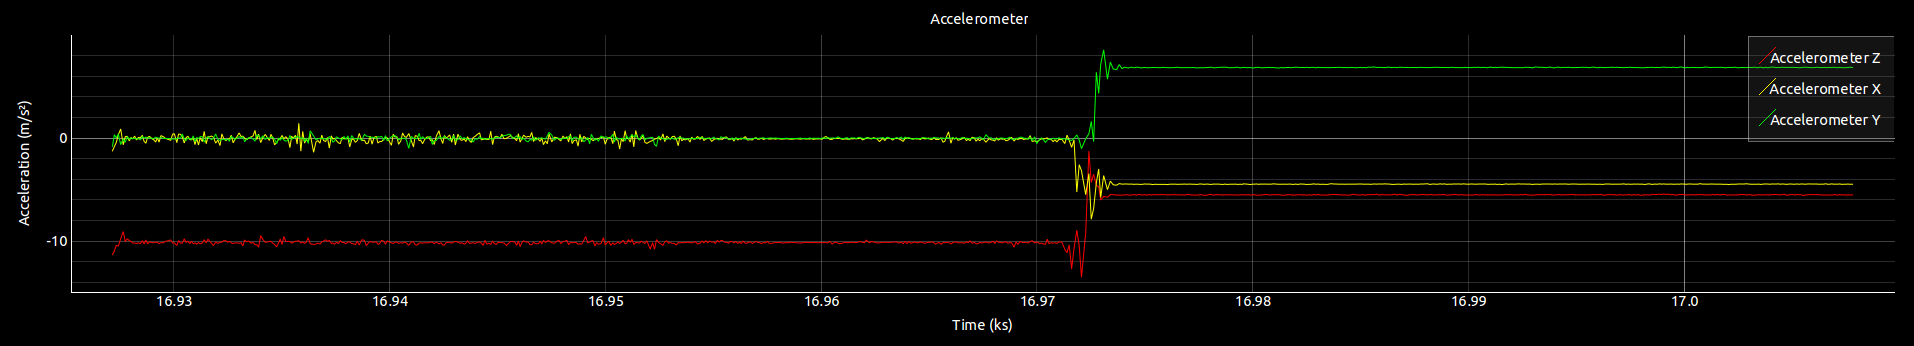
\includegraphics[width=15cm]{images/analyse_1.png}
	\caption{Analyse d'une anomalie: accéléromètre}
	\label{fig:analyse d'une anomalie: accéléromètre}
\end{figure}

\begin{figure}[h]
	\centering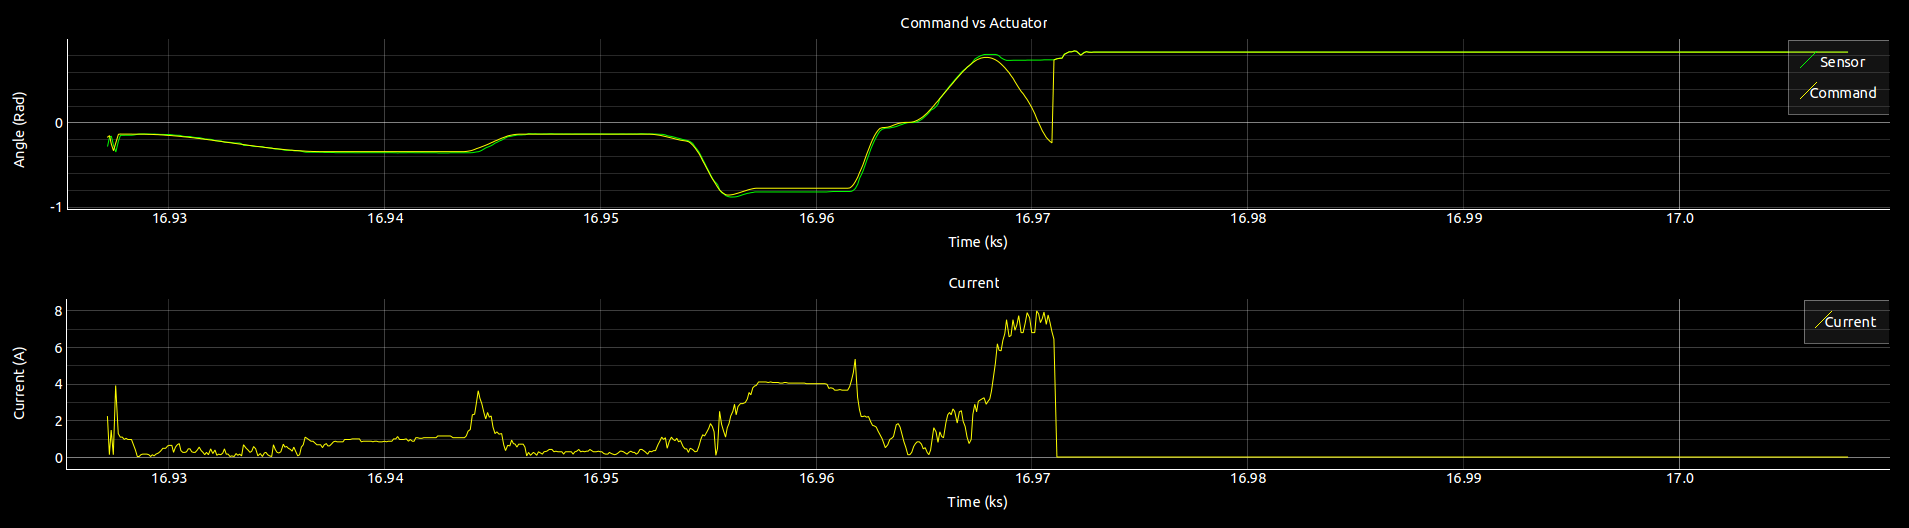
\includegraphics[width=15cm]{images/analyse_2.png}
	\caption{Analyse d'une anomalie: la hanche}
	\label{fig:analyse d'une anomalie: kneePitch}
\end{figure}

\begin{figure}[h]
	\centering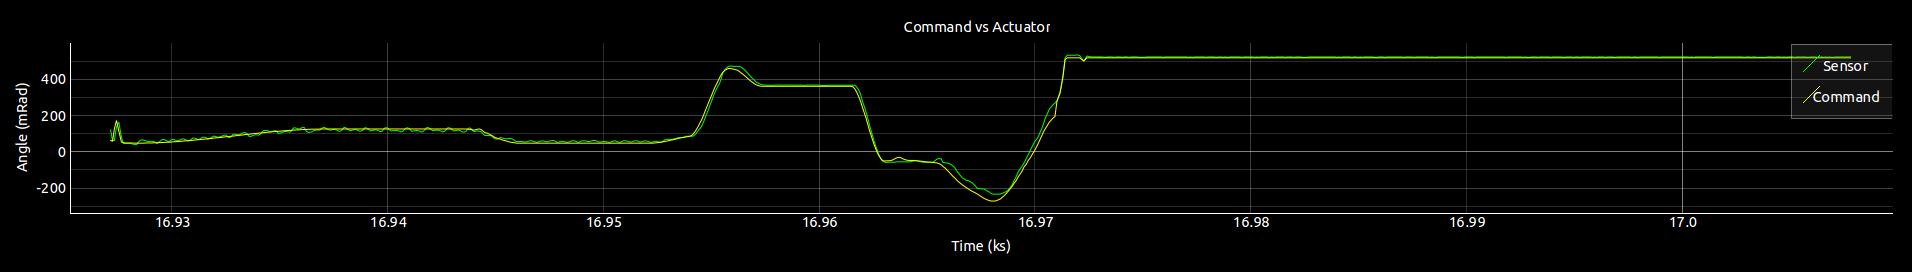
\includegraphics[width=15cm]{images/analyse_3.png}
	\caption{Analyse d'une anomalie: le genou}
	\label{fig:analyse d'une anomalie: hipitch}
\end{figure}

\subsubsection{Hypothèse émise}
 Lors de l'exécution de l'animation "Heat Behavior", le robot est amené à réaliser des mouvements amples au niveau de sa hanche qui causent un certain stress sur cette partie mécanique. Lorsque l'engrenage de la hanche arrive près de sa butée mécanique, un bloquage l'empêche d'atteindre sa position zéro. L'articulation de la hanche ne suit plus sa consigne, ce qui a pour effet de déséquilibrer le robot. Trop déséquilibré, Pepper tombe (\emph{error name}). Une étude plus poussée nous apprendra que la\emph{ root cause } du problème correspondait à un frottement du frein de la hanche. 


\section{Solution proposée}
De part la quantité d'informations à analyser, cette tâche d'analyse peut rapidement devenir rébarbative, d'où le souhait d'automatiser ce processus d'investigation. La variabilité des types de données nous empêche de réduire le nombre d'informations à analyser à de simples caractéristiques communes (e.g. moyenne, écart type, etc.). On s'appuiera donc sur des approches algorithmiques plus poussées, en utilisant notamment des méthodes d'apprentissages automatiques (plus connues sous le terme anglais de Machine Learning). La multiplicité des modèles englobés dans cette discipline nous permettra de répondre au mieux à la problématique.